\chapter{Resoconto attività di verifica}
\section{Analisi statica dei documenti}
Per garantire una buona comprensibilità dei documenti è stato deciso di utilizzare l'\textit{Indice Gulpease} per ottenere una stima della complessità di lettura.
\section{Esiti delle verifiche}
    \subsection{Fino alla prima revisione}
      \subsubsection{Indice Gulpease}  
        \begin{figure}[h!]
            \centering
            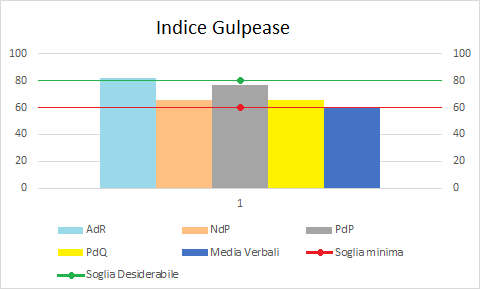
\includegraphics[scale=1.2]{Gulpease.png}
            \caption{Indice di Gulpease per documento}
        \end{figure}
        Come possiamo notare dall'immagine qui sopra tutti i documenti rispettano il valore minimo della metrica MPD2 che il gruppo si è posto come soglia accettabile. L'obiettivo del prossimo periodo sarà portare l'indice di Gulpease sopra soglia desiderabile per tutti i documenti. 
      \subsubsection{Variazione Ore-Costi}  
        \begin{figure}[h!]
            \centering
            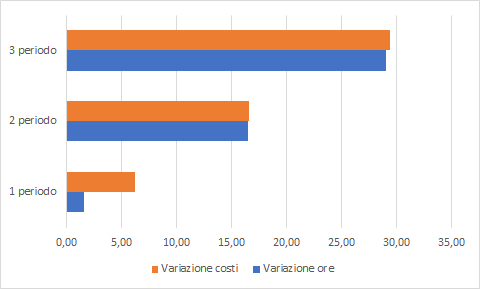
\includegraphics[scale=1.2]{VariazioneOreCosti.png}
            \caption{Variazione delle ore e dei costi}
        \end{figure}
        Dall'immagine è evidente che le variazioni di costi e ore rispetto a quanto preventivato ammontano fino a quasi un 30\% nel periodo 3, ampiamente al di sopra della soglia massima decisa.
